\chapter{Hadron Identification}
\label{cha:hadronID}
%
\section{$\pi^+$ Identification}
\label{sec:pipID}
Positive pions are identified by selecting positive tracks that pass a momentum and sector dependent $\beta$ cut (where $\beta = v/c$).
Additionally, a geometric fiducial cut is applied to region 1 of the DC.
A missing mass cut is also applied.
Traditionally, missing mass cuts are used for selecting particular kinematic regions, not for particle ID.
However, in this situation a missing mass cut significantly improved $\pi^+$/proton separation, and since SIDIS event selection requires a missing mass cut anyway, this cut is applied at the particle ID stage.
%
\subsection{$\pi^+$ Missing Mass Cut}
In pion SIDIS events ($ep \rightarrow e\pi X$), the missing mass ($M_X$) is defined as the invariant mass of the undetected state $X$.
That is, if $p$, $q$, and $\pi$ are the 4-momenta of the initial state proton, the virtual photon, and the detected pion, respectively, then
\begin{equation}
\label{eq:missingMassDefinition}
M_X^2 = \left( p + q - \pi \right)^2.
\end{equation}
To calculate this the pion mass is assumed for the candidate pion.
Figure~\ref{fig:pipMissingMassCut} shows the $M_X$ distribution for candidate $ep \rightarrow e\pi^+ X$ events.
Events with $M_X < 1.35$ GeV are cut.
This cut helps to remove proton contamination at high momenta, which can be seen in figure~\ref{fig:pip_vvp_beforeAndAfter_MXcut} and also cuts out exclusive events ($ep \rightarrow e\pi^+ n$, the peak near the nucleon mass (0.938 GeV) in figure~\ref{fig:pipMissingMassCut}) and the delta resonance (the peak near 1.2 GeV in figure~\ref{fig:pipMissingMassCut}), both of which are not desirable for a SIDIS sample anyway.
\begin{figure}[htp]
\centering
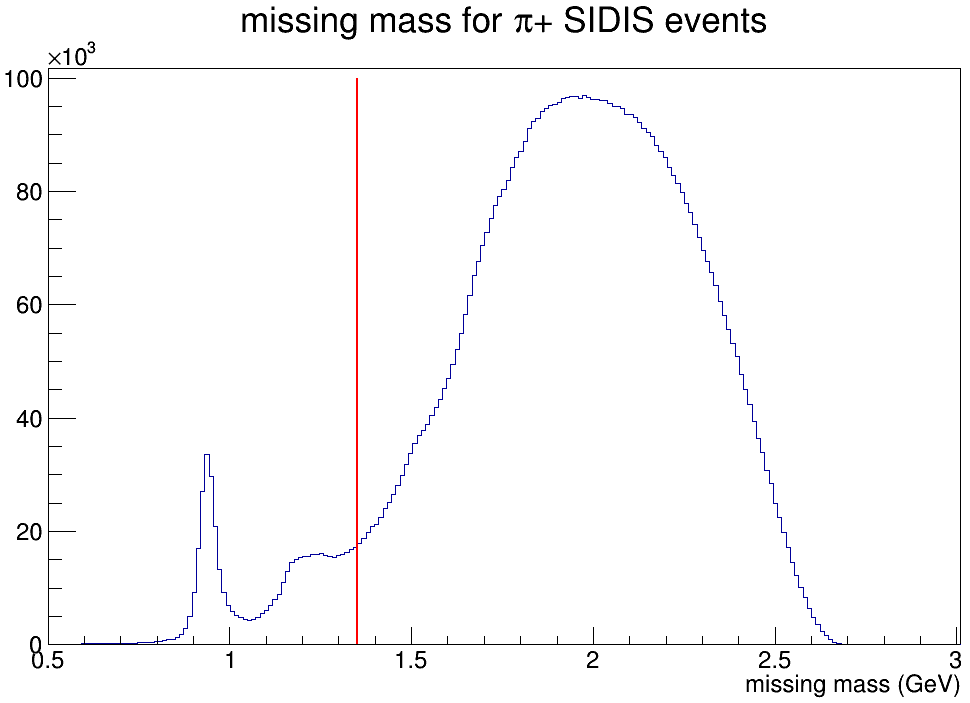
\includegraphics[width=3in]{figures/pipMissingMassCut.png}
\caption{The missing mass distribution for $ep \rightarrow e\pi^+ X$ events. The vertical red line shows the cut of 1.35 GeV. Events to the left of this line are removed from the sample.}
\label{fig:pipMissingMassCut}
\end{figure}
%
\begin{figure}[htp]
\centering
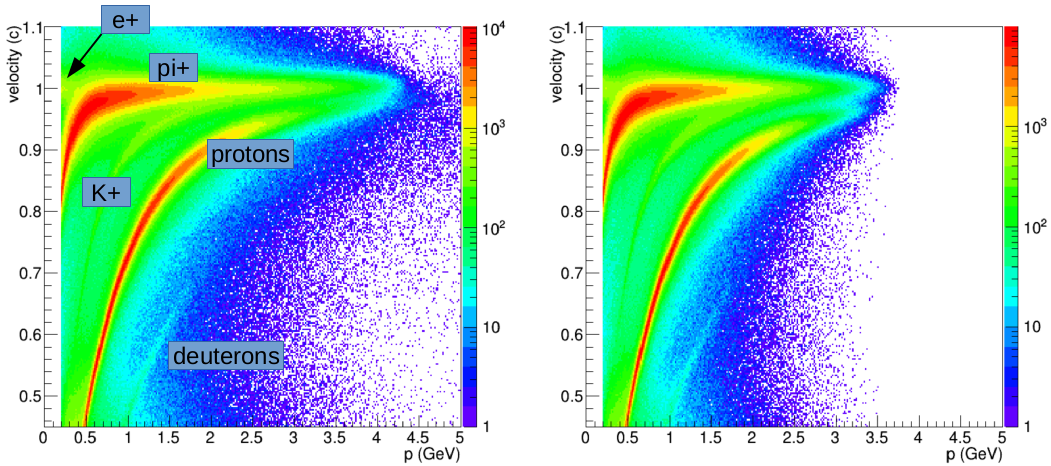
\includegraphics[width=6in]{figures/pip_vvp_beforeAndAfter_MXcut.png}
\caption{$\beta$ vs momentum distribution for positive tracks before (left) and after (right) the missing mass cut. The cut removes most tracks above 3.5 GeV, making $\pi^+$/proton separation easier. SIDIS samples require a missing mass cut anyway, so it makes sense to apply it here at the particle ID stage.}
\label{fig:pip_vvp_beforeAndAfter_MXcut}
\end{figure}
%
\subsection{$\pi^+ \beta$ Cut}
$\beta$ is calculated by simply dividing the track's path length by its time of flight and then dividing this quantity by the speed of light.
To select positive pions, $\beta$ for positive tracks is plotted in 70 bins of momentum from 0.2 to 3.75 GeV (with the missing mass cut applied).
The pion peak for each bin is then fit with a gaussian.
At low momenta, a $3\sigma$ cut is used, while at higher momenta a tighter cut, which was estimated by eye, is used.
The tightening of the cut at higher momenta is clearly necessary to reduce proton contamination.
This is shown (for electron sector 4) in figure~\ref{fig:pos_1Dbeta_pBins} - the top left plot is the lowest momentum bin and the bottom right plot highest momentum bin, the red curves show the gaussian fits, the vertical black lines show $\mu \pm 3\sigma$, and the vertical red lines show the actual cut.
The two dimensional view of this cut is shown in figure~\ref{fig:pip_vvpCut}.
%
\begin{sidewaysfigure}[htp]
\centering
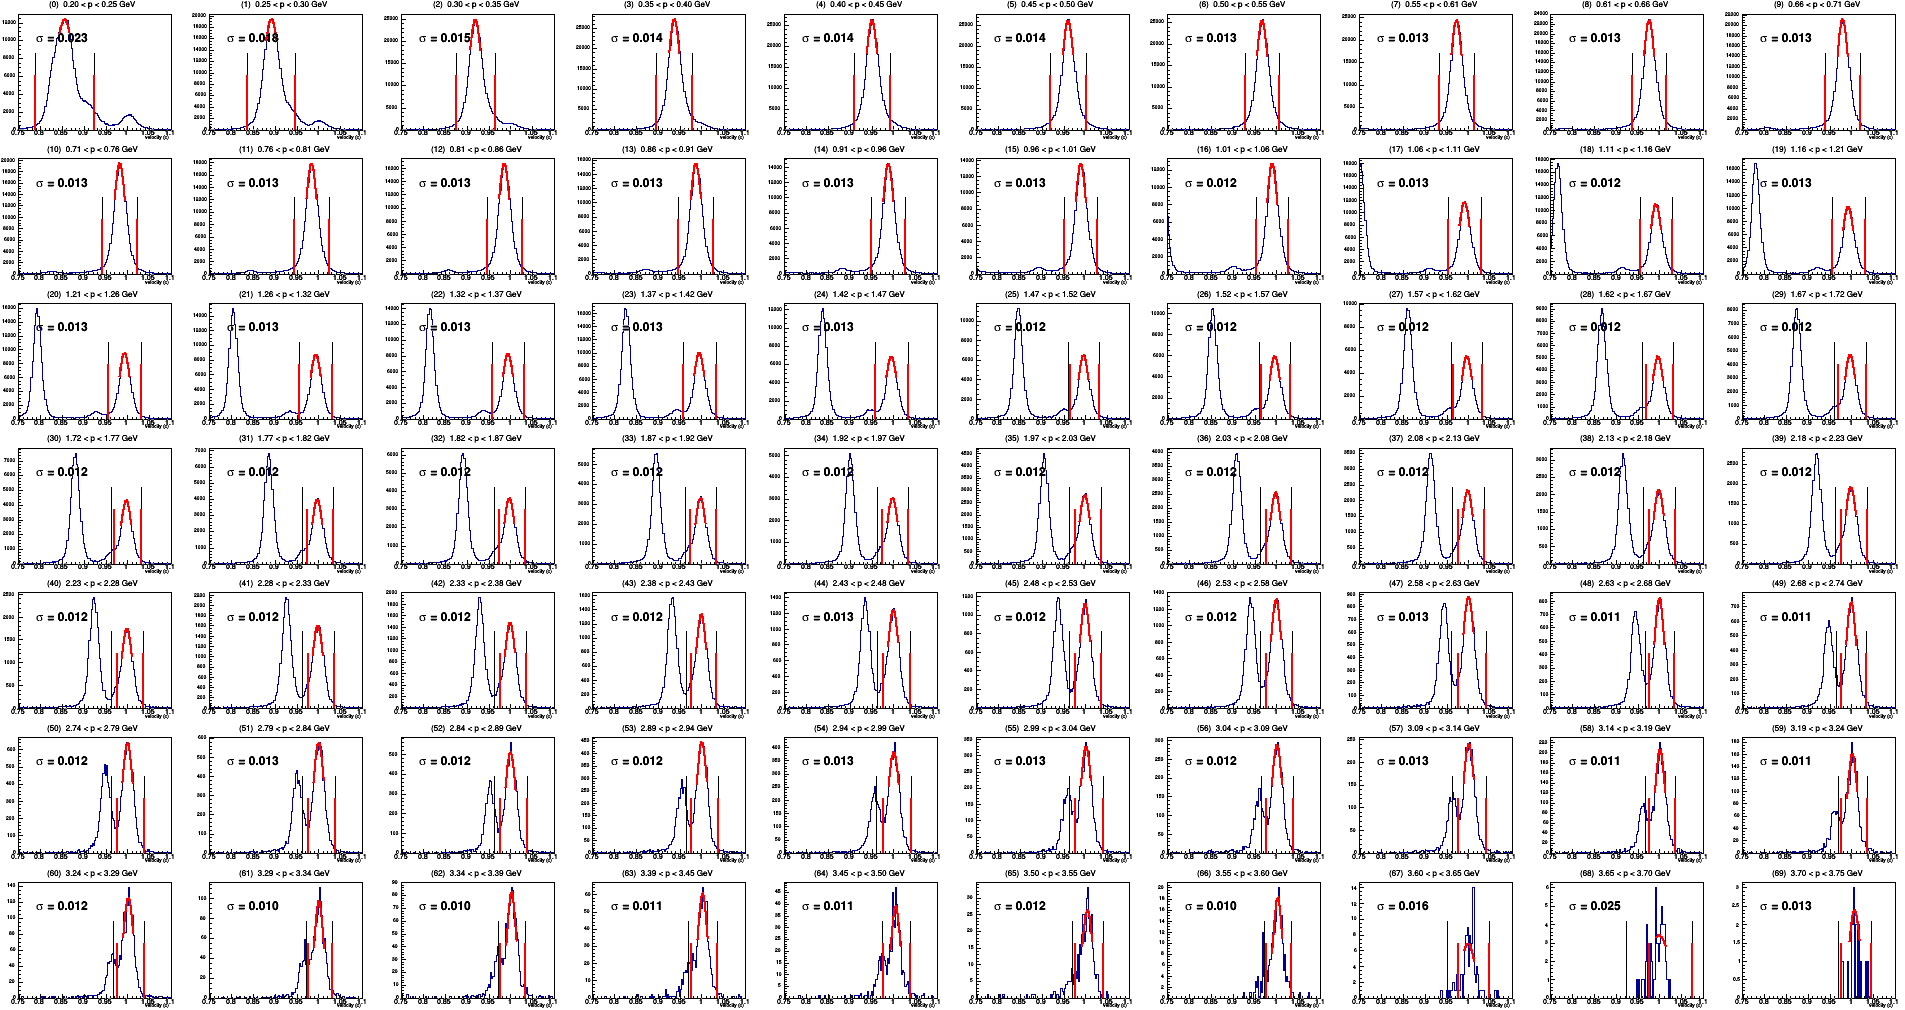
\includegraphics[width=8.5in]{figures/pos_1Dbeta_pBins.png}
\caption{$\beta$ for positive tracks in bins of momentum when the electron is in sector 4. The top left plot is the lowest momentum bin and the bottom right plot highest momentum bin, the red curves show the gaussian fits, the vertical black lines show $\mu \pm 3\sigma$, and the vertical red lines show the actual cut.}
\label{fig:pos_1Dbeta_pBins}
\end{sidewaysfigure}
%
\begin{figure}[htp]
\centering
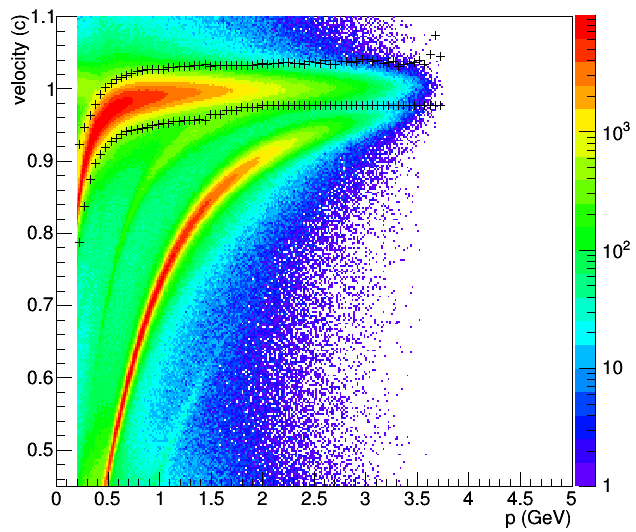
\includegraphics[width=4in]{figures/pip_vvpCut.png}
\caption{The two dimensional view of the $\pi^+$ $\beta$ cut. The black crosses show the upper and lower cut for each of the 70 momentum bins.}
\label{fig:pip_vvpCut}
\end{figure}
%
\subsection{$\pi^+$ Fiducial Cut}
To improve the data quality, a geometric fiducial cut is applied to region 1 of the DC.
The cut is shown with red lines in figure~\ref{fig:pip_R1cut_s4}.
The lines are symmetric and form a $60^\circ$ angle and intersect at $(0, 10)$ cm.
\begin{figure}[htp]
\centering
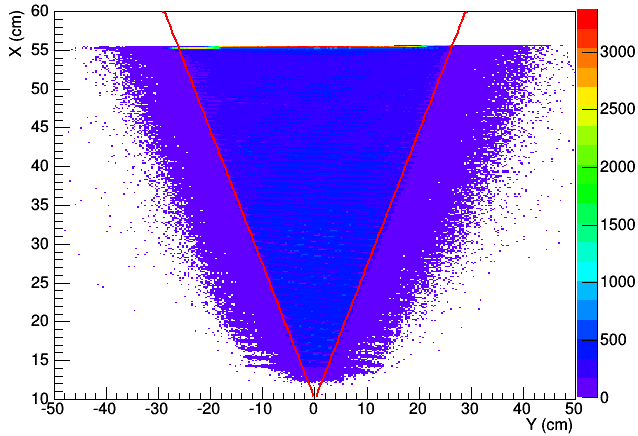
\includegraphics[width=4in]{figures/pip_R1cut_s4.png}
\caption{X vs Y in region 1 of the DC for positive tracks. Events inside of the red lines are kept.}
\label{fig:pip_R1cut_s4}
\end{figure}
%
%

\clearpage % should prevent a backlog of figures from piling up

%
%
\section{$\pi^-$ Identification}
\label{sec:pimID}
Negative tracks that are not identified as electrons become $\pi^-$ candidates.
Negative pions are then selected using cuts very similar to the $\pi^+$ ID.
%
\subsection{$\pi^-$ Missing Mass Cut}
Although the $\pi^-$ channel does not have proton (or anti-proton) contamination, a missing mass cut of 1.35 GeV is applied here as well for consistency.
Figure~\ref{fig:pimMissingMassCut} shows this cut.
%
\begin{figure}[htp]
\centering
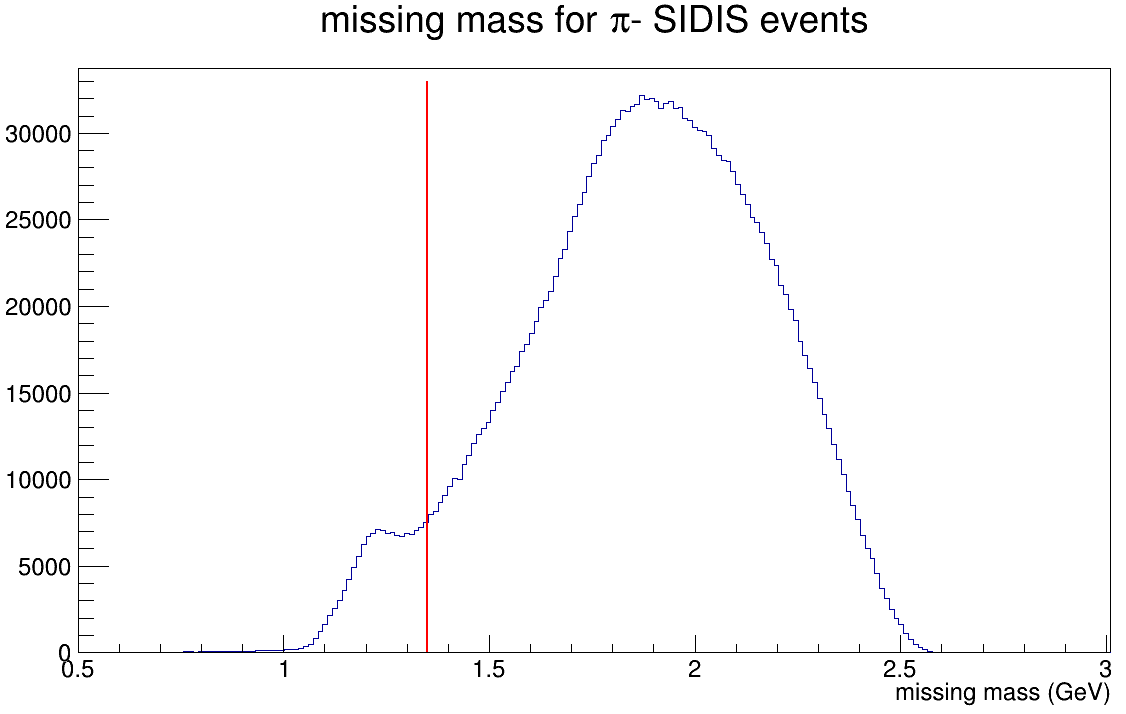
\includegraphics[width=3in]{figures/pimMissingMassCut.png}
\caption{The missing mass distribution for $ep \rightarrow e\pi^- X$ events. The vertical red line shows the cut of 1.35 GeV. Events to the left of this line are removed from the sample.}
\label{fig:pimMissingMassCut}
\end{figure}
%
\subsection{$\pi^- \beta$ Cut}
The $\pi^-$ $\beta$ cut is done in exactly the same way as $\pi^+$ $\beta$ cut.
The results can be seen in figures~\ref{fig:neg_1Dbeta_pBins} and~\ref{fig:pim_vvpCut}.
%
\begin{sidewaysfigure}[htp]
\centering
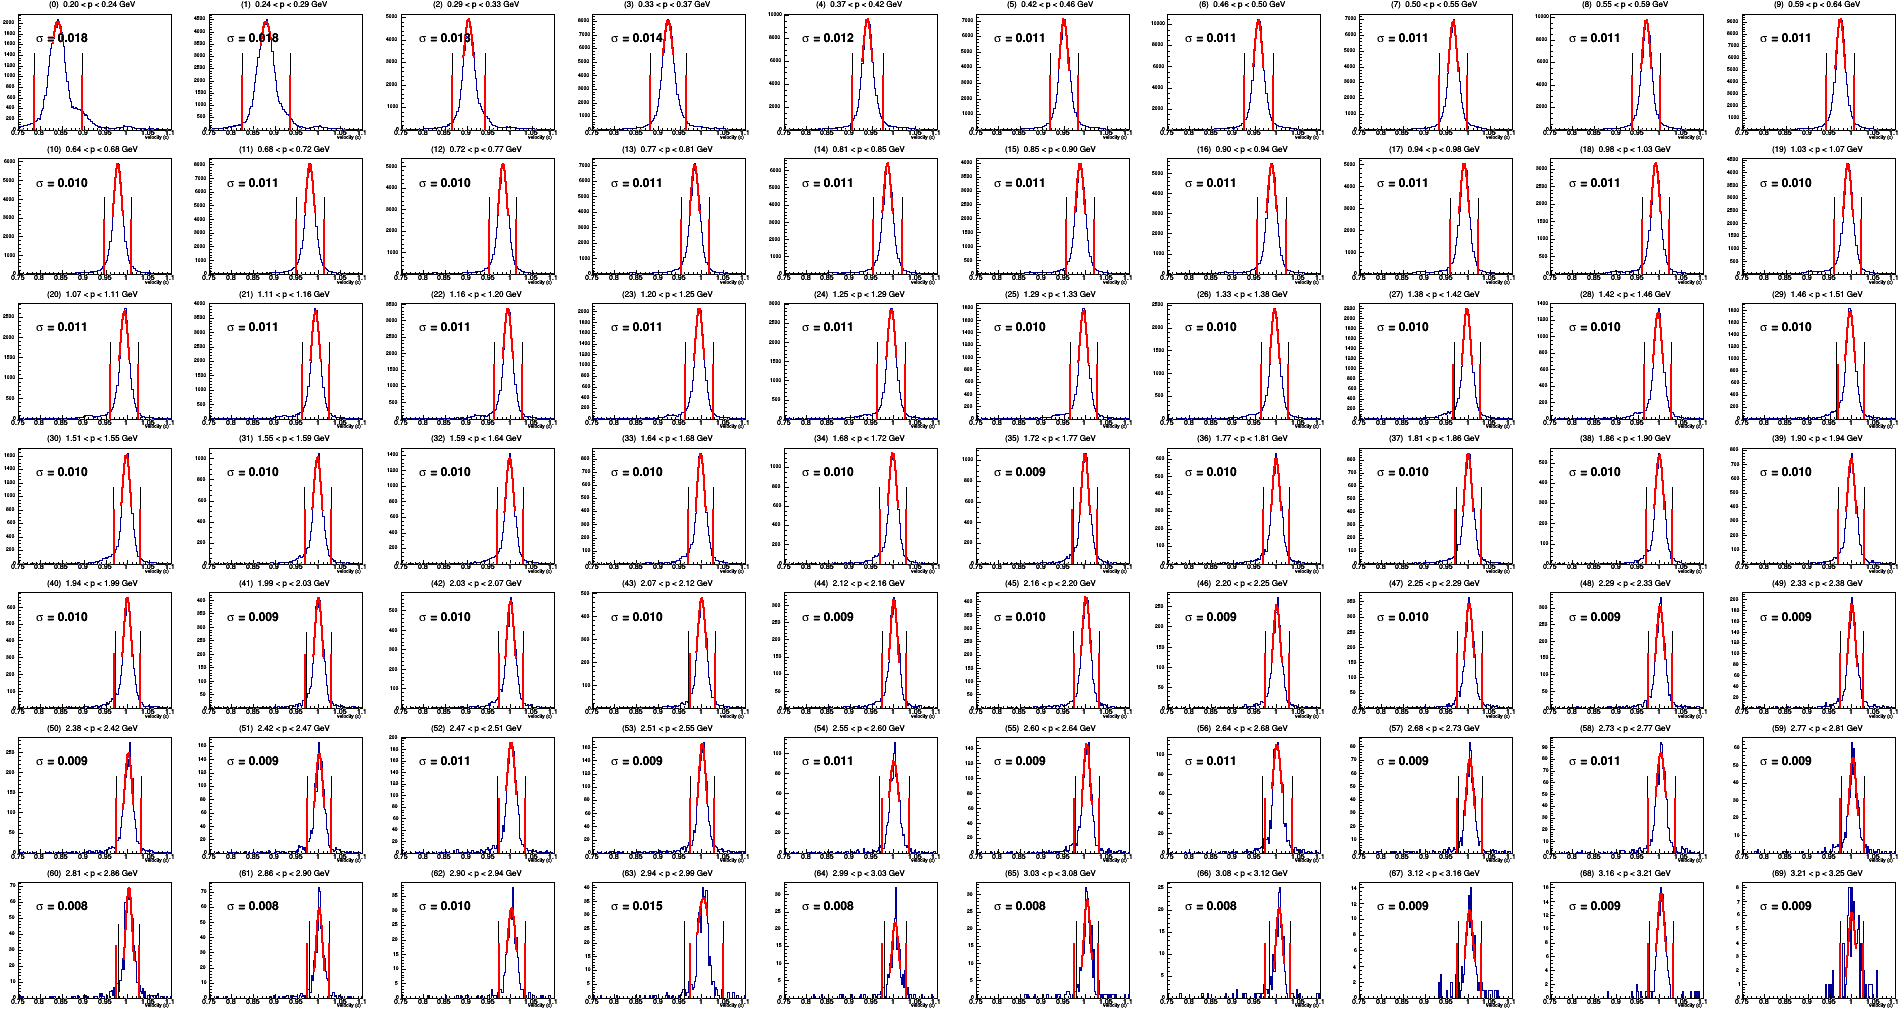
\includegraphics[width=8.5in]{figures/neg_1Dbeta_pBins.png}
\caption{$\beta$ for negative tracks in bins of momentum when the electron is in sector 3. The top left plot is the lowest momentum bin and the bottom right plot highest momentum bin, the red curves show the gaussian fits, the vertical black lines show $\mu \pm 3\sigma$, and the vertical red lines show the actual cut.}
\label{fig:neg_1Dbeta_pBins}
\end{sidewaysfigure}
%
\begin{figure}[htp]
\centering
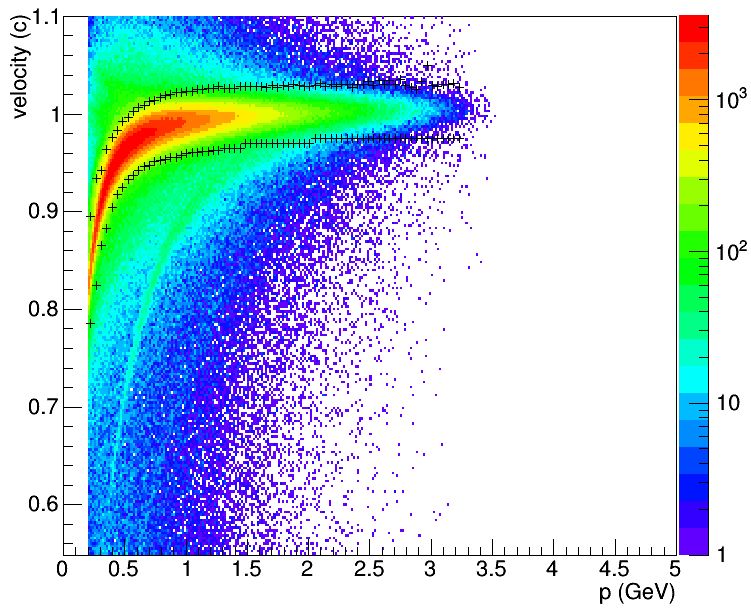
\includegraphics[width=4in]{figures/pim_vvpCut.png}
\caption{The two dimensional view of the $\pi^-$ $\beta$ cut. The black crosses show the upper and lower cut for each of the 70 momentum bins.}
\label{fig:pim_vvpCut}
\end{figure}
%
%
\subsection{$\pi^-$ Fiducial Cut}
To improve the data quality, a geometric fiducial cut is applied to region 1 of the DC.
The cut is shown with red lines in figure~\ref{fig:pim_R1cut_s4}.
The diagonal lines are symmetric and form an $80^\circ$ angle and intersect at $(0, 20)$ cm.
The horizontal line is at X = 24 cm.
\begin{figure}[htp]
\centering
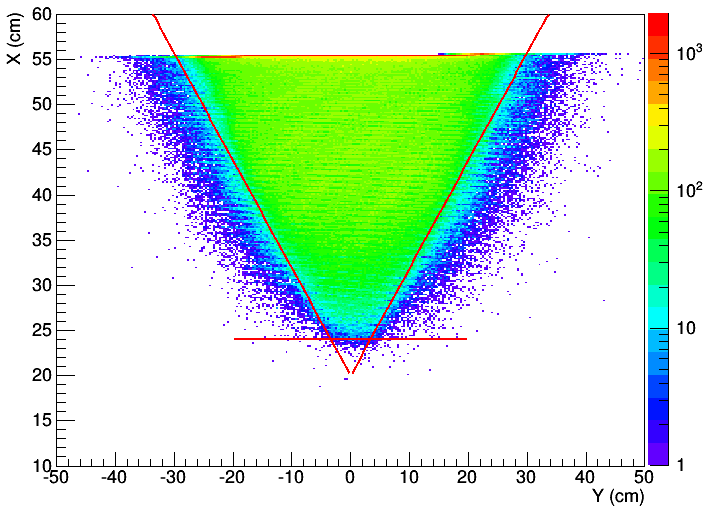
\includegraphics[width=4in]{figures/pim_R1cut_s4.png}
\caption{X vs Y in region 1 of the DC for negative tracks. Events inside of the red lines are kept.}
\label{fig:pim_R1cut_s4}
\end{figure}
%


